\section{The READEX Methodology} \label{sec:methodology}

The READEX methodology is split into two phases: design-time (during application development) and runtime (during production runs). READEX performs a sequence of steps to produce tuning advice for an application. The following sections describe the steps defined in the READEX methodology.

%\begin{figure}[!t]
%\centering
%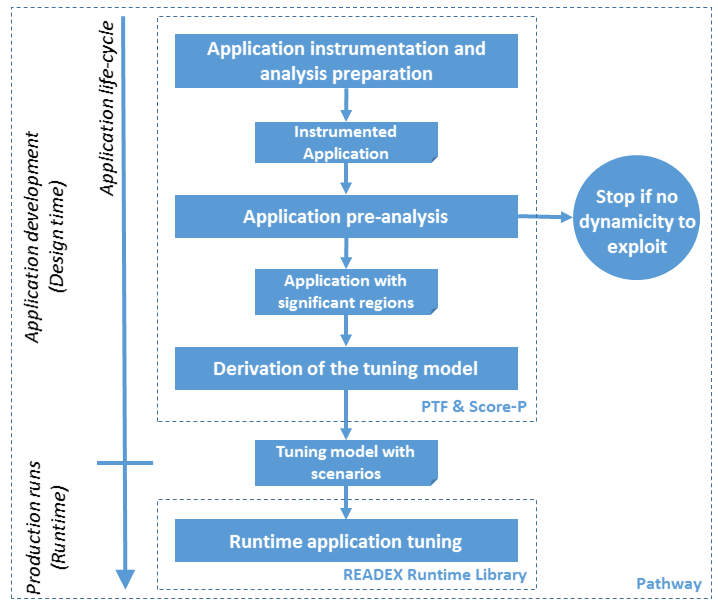
\includegraphics[width=.70\columnwidth]{figures/READEX_workflow.png}
%\caption{Overview of READEX methodology}
%\label{fig:readex_methodology}
%\end{figure}

\subsection{Application Instrumentation and Analysis Preparation}
\label{sec:application_instrumentation}
The first step in READEX is to instrument the HPC application by inserting probe-functions around different regions that are of interest to tuning. A region can be any arbitrary part of the code, for instance a function or a loop. READEX is based on instrumentation with Score-P and requires that the \textit{phase region} is manually annotated. The phase region is the body of the main progress loop of the application. In addition to the phase region, READEX supports instrumentation of \textit{user regions} using Score-P.

The READEX methodology also allows specifying domain knowledge in the form of additional identifiers for rts's. This allows to distinguish rts's of the same region and assign different optimal configurations. For example, an identifier can determine the grid level in a multigrid program, and thus different configurations can be assigned for the relaxation operation executed on the different levels. 

\subsection{Application Pre-analysis}
\label{sec:dynamism_detection}
After instrumenting an application and preparing it for analysis, the second step in the READEX approach is to perform a pre-analysis. The objective of this step is to automatically identify and characterize dynamism in the application behaviour. This is critical because the READEX approach is based on tuning hardware, system and application parameters, depending on the dynamism exhibited by the different regions in the application. READEX is capable of identifying and characterizing two types of application dynamism:
\begin{itemize}
  \item \textit{Inter-phase dynamism}: This occurs if different instances of the phase region have different execution characteristics. This might lead to different optimal configurations.
  \item \textit{Intra-phase dynamism}: This occurs rts's executed during a single phase have different characteristics, e.g., invocations of different subroutines.
\end{itemize}

The pre-analysis also identifies coarse-granular regions that have enough internal computation to rectify the overhead for switching configurations. These regions are called \textit{significant regions}. 

If no dynamism is identified in the pre-analysis, the rest of the READEX steps are aborted due to the homogeneous behaviour of the application, which will not yield any energy or performance savings from auto-tuning.

Listing \ref{lst:minimd_dynamism_summary} presents an example of the summary of significant regions and the dynamism identified by READEX in the miniMD application.

\lstset{language=[90]Fortran,
	basicstyle=\ttfamily\scriptsize,
	frame=tb,
	aboveskip=2mm,
	belowskip=2mm,
	showstringspaces=false,
	columns=flexible,
	breaklines=true,
	breakatwhitespace=true,
	keywordstyle=\color{black},
	commentstyle=\color{black},
	escapeinside={(@*}{*@)},
}

\begin{figure}[!t]
\centering
\begin{lstlisting}
...
Significant regions are:

void Comm::borders(Atom&)
void ForceLJ::compute_halfneigh(Atom&, Neighbor&, int) [with int EVFLAG = 0; int GHOST_NEWTON = 1]
void ForceLJ::compute_halfneigh(Atom&, Neighbor&, int) [with int EVFLAG = 1; int GHOST_NEWTON = 1]
void Neighbor::build(Atom&)

Significant region information
==============================
Region name                  Min(t)          Max(t)       Time Dev.(%Reg) Ops/L3miss    Weight(%Phase)

void Comm::borders(Atom&)    0.001             0.001            2.6           109              0
void ForceLJ::compute_hal    0.013             0.014            2.9            97             68
void ForceLJ::compute_hal    0.016             0.016            0.0            91              1
void Neighbor::build(Atom    0.047             0.048            0.7           332             23


Phase information
=================
Min                  Max                  Mean                 Dev.(% Phase)        Dyn.(% Phase)

0.0138626            0.0664566            0.020337             72.731               258.612

...

SUMMARY:
========

Inter-phase dynamism due to variation of execution time of phases

No intra-phase dynamism due to time variation

Intra-phase dynamism due to variation in compute intensity of following significant regions

void ForceLJ::compute_halfneigh(Atom&, Neighbor&, int) [with int EVFLAG = 0; int GHOST_NEWTON = 1]
void Neighbor::build(Atom&)
\end{lstlisting}
\caption{Summary of the application pre-analysis for miniMD. Significant intra-phase dynamism due to variation in the compute intensity was found for \texttt{compute\_halfneigh()} and \texttt{build()}. In addition, inter-phase dynamism was observed for the phase region due to variation in the execution time.}
\label{fig:pre-analysisOutput}
\end{figure}

\subsection{Derivation of Tuning Model}
\label{sec:tuning_model_generation}

Following the identification of exploitable dynamism in the pre-analysis step, the third step explores the space of possible tuning configurations, and identifies the optimal configurations of the tuning parameters for the phases and rts's during the application execution. This analysis is performed by PTF (Periscope Tuning Framework) in conjunction with Score-P and the RRL (READEX Runtime Library). PTF performs DTA experiments through a number of possible search strategies, such as exhaustive, individual, and heuristic search based on generic algorithm to identify the optimal configurations for the rts's of the significant regions identified in the pre-analysis step. To achieve this, Score-P provides the instrumentation and profiling platform, while the RRL provides the platform for libraries to tune hardware and system parameters. Additionally, READEX also has dedicated libraries that tune application-specific parameters.

It is important to note that the additional identifiers, which can be specified during the instrumentation step provide additional domain knowledge to distinguish and identify different optimal configurations for runtime scenarios~\cite{PACO17}.

After all experiments are completed and optimal configurations are identified, the rts's are grouped into a limited number of scenarios, e.g., up to 20. Each scenario is associated with a common system configuration, and it is hence composed of rts's with identical or similar best configurations. The limitation in the number of scenarios inhibits a too frequent configuration switching at runtime that may result in higher overheads from auto-tuning. The set of scenarios, information about the rts's associated with the scenarios, and the optimal configurations for each scenario are stored by PTF in the form of a serialized text file called the Application Tuning Model (ATM), which is loaded and exploited during production runs at runtime.

\subsection{Runtime Application Tuning}
\label{sec:runtime_tuning}

Following the completion of DTA, production runs of the application can now be tuned at runtime using the optimal configurations summarized in the ATM using the RRL. The RRL monitors the application execution using the Score-P instrumentation, identifies the scenario that is encountered at runtime, and applies the corresponding optimal configurations for each scenario using the knowledge in the ATM to optimize the application's energy consumption. The RRL uses libraries that are loaded as plugins for setting different configurations of the tuning parameters.

\subsection{Pathway for READEX Workflow}
\label{sec:pathway_for_readex_workflow}

Since the READEX methodology has quite a number of steps, it uses Pathway to automate the entire workflow. Pathway \cite{Pathway:Petkov13} is a tool for designing and executing performance engineering workflows for HPC applications. Pathway provides an out-of-the box workflow template that can be configured to apply READEX on an application in an HPC system of choice. This way, Pathway can keep track of each step that must be completed in order to obtain the tuning results. Figure~\ref{fig:pathway_browser} presents an example of a custom browser in Pathway that summarizes the results from each step of applying READEX on the miniMD application. The left pane shows the tuned applications. The top pane shows a list of experiments performed with the READEX workflow. The middle pane shows the results from the pre-analysis step, describing the dynamism detected in the application. The bottom pane displays the ATM containing the tuning results.

%\begin{figure}[!t]
%\centering
%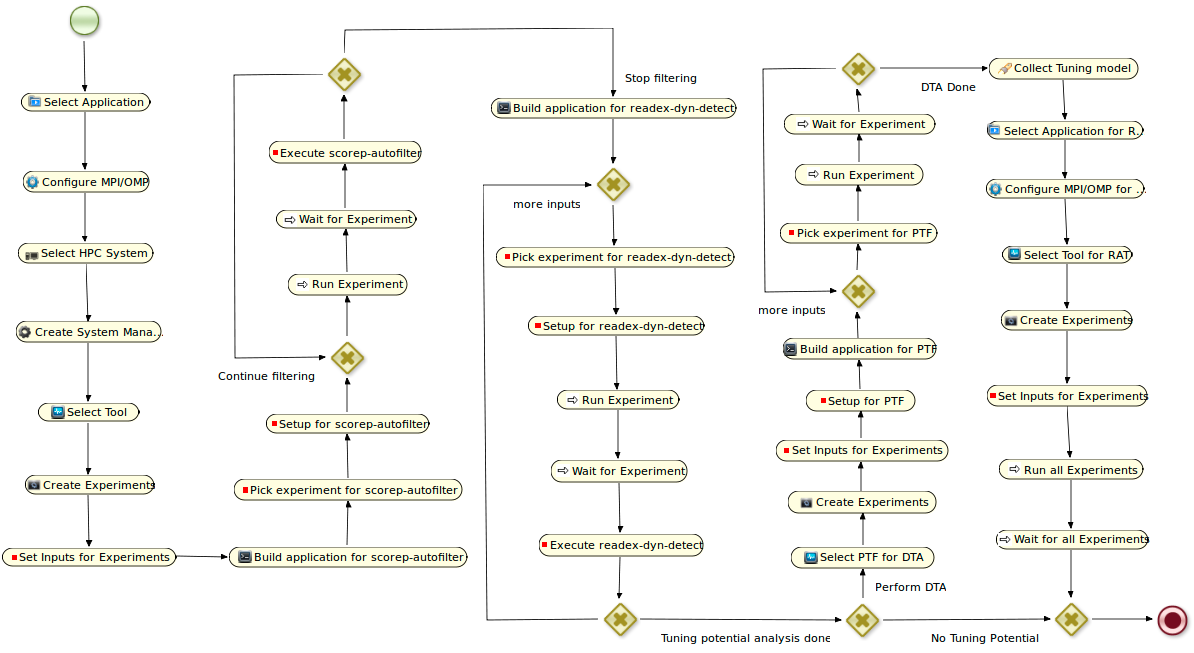
\includegraphics[width=.95\columnwidth]{figures/PathwayWorkflow.png}
%\caption{READEX Workflow in Pathway}
%\label{fig:pathway_workflow}
%\end{figure}

\begin{figure}[!t]
\centering
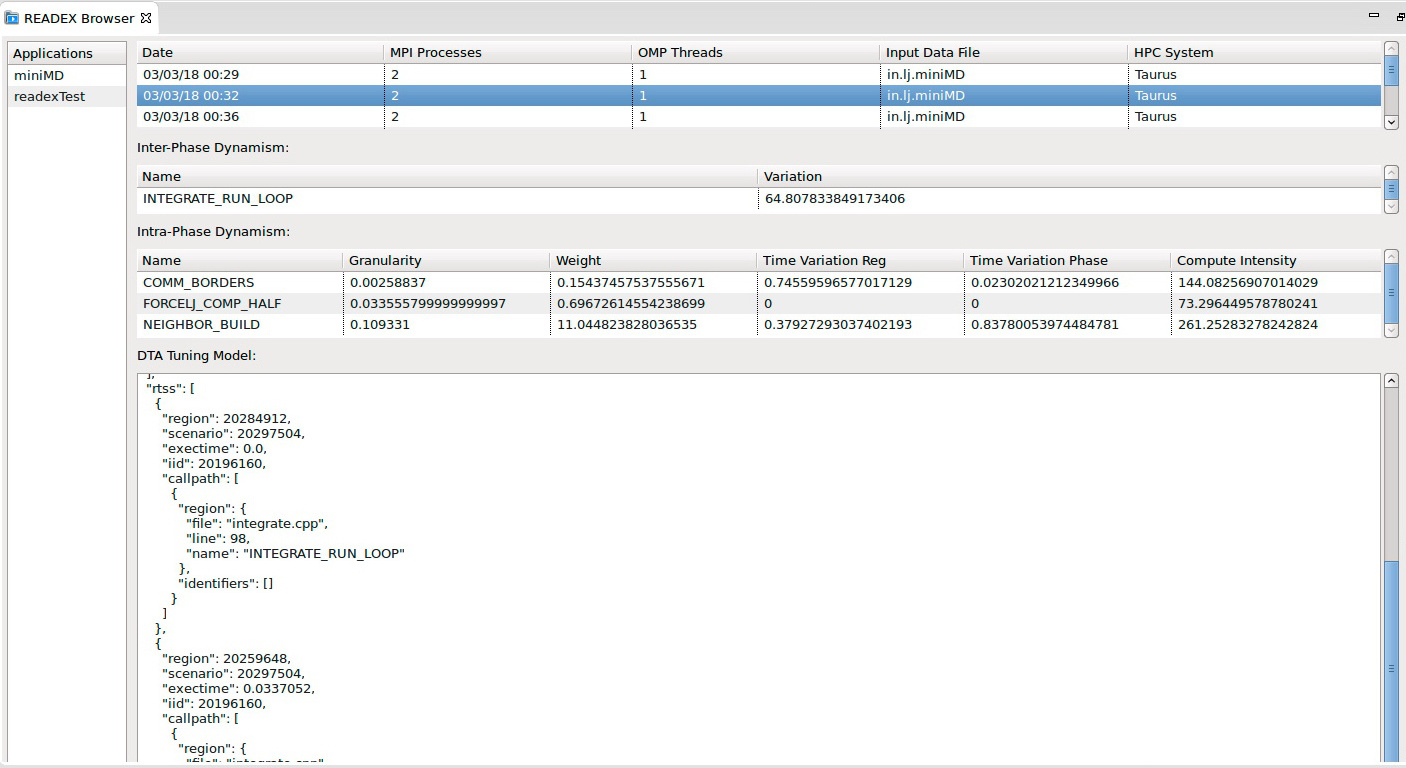
\includegraphics[width=.95\columnwidth]{figures/PathwayBrowser.jpeg}
\caption{READEX Results Browser in Pathway}
\label{fig:pathway_browser}
\end{figure}
